\documentclass{beamer}

\mode<presentation> {
  \usetheme{Madrid}
  % \setbeamercovered{transparent}
  \setbeamertemplate{navigation symbols}{}
}

\usepackage{amsmath,amssymb,empheq}
\usepackage{color}
\usepackage[T1]{fontenc}
\usepackage{graphicx}
\usepackage[utf8]{inputenc}
\usepackage{pgfplots}
\usepackage{svg} % IMPORTANT NOTE: Images in the SVG format should be sized at 450x280px
\usepackage{tikz}

\graphicspath{{images/}}

\setsvg{inkscape=inkscape -z -C,svgpath=images/}

\newcommand{\AutoSectionTitle}{}


%% TITLE PAGE %%%%%%%%%%%%%%%%%%%%%%%%%%%%%%%%%%%%%%%%%%%%%%%%%%%%%%%%%%%%%%%%%%%%%%%%%%%%%%%%%%%%%%


\title[Comparison of Optimization Methods]{A Comparison of Optimization Methods for Multi-Objective Constrained Bin Packing Problems}

\author[P. Olivier, A. Lodi, G. Pesant] {
  P. Olivier$^1$, A. Lodi$^1$, G. Pesant$^1$ \\
  \vspace{0.5cm}
  \scriptsize $^1$École polytechnique de Montréal, Montreal, Canada \\
  \{philippe.olivier, andrea.lodi, gilles.pesant\}@polymtl.ca \\
  \vspace{1cm}
  \normalsize JOPT 2018
}

\date[JOPT 2018]{8 May 2018}

\begin{document}

\begin{frame}
  \titlepage
\end{frame}

\begin{frame}
  \frametitle{Outline}
  \tableofcontents
\end{frame}


%% THE WEDDING SEATING PROBLEM %%%%%%%%%%%%%%%%%%%%%%%%%%%%%%%%%%%%%%%%%%%%%%%%%%%%%%%%%%%%%%%%%%%%%


\renewcommand{\AutoSectionTitle}{The Wedding Seating Problem}

\section{\AutoSectionTitle}

\begin{frame}
  \frametitle{Outline}
  \tableofcontents[currentsection]
\end{frame}


%---------------------------------------------------------------------------------------------------


\begin{frame}
  \frametitle{\AutoSectionTitle}
  
  \begin{center}
    \includesvg{wsp_groups_and_tables}
  \end{center}
  
\end{frame}


%---------------------------------------------------------------------------------------------------


\begin{frame}
  \frametitle{\AutoSectionTitle}
  
  \begin{center}
    \includesvg{wsp_groups_seated}
  \end{center}
  
\end{frame}


%---------------------------------------------------------------------------------------------------


\begin{frame}
  \frametitle{\AutoSectionTitle}
  
  \begin{center}
    \includesvg{wsp_relations0}
  \end{center}
  
\end{frame}


%---------------------------------------------------------------------------------------------------


\begin{frame}
  \frametitle{\AutoSectionTitle}
  
  \begin{center}
    \includesvg{wsp_relations1}
  \end{center}
  
\end{frame}


%---------------------------------------------------------------------------------------------------


\begin{frame}
  \frametitle{\AutoSectionTitle}
  
  \begin{center}
    \includesvg{wsp_relations2}
  \end{center}
  
\end{frame}


%---------------------------------------------------------------------------------------------------


\begin{frame}
  \frametitle{\AutoSectionTitle}
  
  \begin{center}
    \includesvg{wsp_relations3}
  \end{center}
  
\end{frame}


%---------------------------------------------------------------------------------------------------


\begin{frame}
  \frametitle{\AutoSectionTitle}
  
  \begin{center}
    \includesvg{wsp_relations4}
  \end{center}
  
\end{frame}


%---------------------------------------------------------------------------------------------------


\begin{frame}
  \frametitle{\AutoSectionTitle}
  
  \begin{center}
    \includesvg{wsp_balanced_tables}
  \end{center}
  
\end{frame}


%% EXISTING METHODS %%%%%%%%%%%%%%%%%%%%%%%%%%%%%%%%%%%%%%%%%%%%%%%%%%%%%%%%%%%%%%%%%%%%%%%%%%%%%%%%


\renewcommand{\AutoSectionTitle}{Existing Methods}

\section{\AutoSectionTitle}

\begin{frame}
  \frametitle{Outline}
  \tableofcontents[currentsection]
\end{frame}


%---------------------------------------------------------------------------------------------------


\begin{frame}
  \frametitle{\AutoSectionTitle}
  \framesubtitle{Overview}
  
  \begin{itemize}
  \item Original IP model [Bellows and Petersen, \emph{Annals of Improbable Research}, 2012]. \\~\\
  \item Two-stage algorithm using tabu search [Lewis, \emph{WorldComp International Conference Proceedings}, 2013]. \\~\\
  \item Improved IP model [Lewis and Carroll, \emph{Journal of the Operational Research Society}, 2016].
  \end{itemize}
  
\end{frame}


%---------------------------------------------------------------------------------------------------


\begin{frame}
  \frametitle{\AutoSectionTitle}
  \framesubtitle{Two-stage algorithm using tabu search [Lewis, 2013]}
  
  Build a graph where nodes represent groups, edges represent relations, and colors represent tables. \\~\\

  \pause

  \begin{itemize}
  \item Stage 1: Color nodes to find an initial feasible solution \\~\\
    
    \pause
    
  \item Stage 2: Improve this feasible solution with a tabu search
  \end{itemize}
  
\end{frame}


%% CP MODEL %%%%%%%%%%%%%%%%%%%%%%%%%%%%%%%%%%%%%%%%%%%%%%%%%%%%%%%%%%%%%%%%%%%%%%%%%%%%%%%%%%%%%%%%


\renewcommand{\AutoSectionTitle}{CP Model}

\section{\AutoSectionTitle}

\begin{frame}
  \frametitle{Outline}
  \tableofcontents[currentsection]
\end{frame}


%---------------------------------------------------------------------------------------------------


\begin{frame}
  \frametitle{\AutoSectionTitle}
  
  \begin{center}
    \includesvg{cp_conflict_graph1}
  \end{center}
  
\end{frame}


%---------------------------------------------------------------------------------------------------


\begin{frame}
  \frametitle{\AutoSectionTitle}
  
  \begin{center}
    \includesvg{cp_conflict_graph2}
  \end{center}
  
\end{frame}


%---------------------------------------------------------------------------------------------------


\begin{frame}
  \frametitle{\AutoSectionTitle}
  
  \begin{center}
    \includesvg{cp_model1}
  \end{center}
  
\end{frame}


%---------------------------------------------------------------------------------------------------


\begin{frame}
  \frametitle{\AutoSectionTitle}
  
  \begin{center}
    \includesvg{cp_model2}
  \end{center}
  
\end{frame}


%---------------------------------------------------------------------------------------------------


\begin{frame}
  \frametitle{\AutoSectionTitle}
  
  \begin{center}
    \includesvg{cp_model3}
  \end{center}
  
\end{frame}


%---------------------------------------------------------------------------------------------------


\begin{frame}
  \frametitle{\AutoSectionTitle}
  
  \begin{center}
    \includesvg{cp_model4}
  \end{center}
  
\end{frame}


%---------------------------------------------------------------------------------------------------


\begin{frame}
  \frametitle{\AutoSectionTitle}
  
  \begin{center}
    \includesvg{cp_model5}
  \end{center}
  
\end{frame}


%---------------------------------------------------------------------------------------------------


\begin{frame}
  \frametitle{\AutoSectionTitle}
  \framesubtitle{Branching and Search}
  
  Branching heuristic (similar to \emph{best fit decreasing}): \\

  \begin{enumerate}
  \item Pick the largest group yet unassigned \\
  \item Assign that group at the best possible table \\
  \item If no table has enough room, open a new table \\~\\~\\
  \end{enumerate}

  \pause

  Large Neighborhood Search (LNS):

  \begin{itemize}
  \item Freeze $\sim$1/3 of the tables for 10s \\
  \item The best tables are more likely to be frozen
  \end{itemize}
  
\end{frame}


%% IP MODEL A %%%%%%%%%%%%%%%%%%%%%%%%%%%%%%%%%%%%%%%%%%%%%%%%%%%%%%%%%%%%%%%%%%%%%%%%%%%%%%%%%%%%%%


\renewcommand{\AutoSectionTitle}{IP Model A}

\section{\AutoSectionTitle}

\begin{frame}
  \frametitle{Outline}
  \tableofcontents[currentsection]
\end{frame}


%---------------------------------------------------------------------------------------------------


\begin{frame}
  \frametitle{\AutoSectionTitle}

  \uncover<1->{
    \begin{equation*}
      x_{ik}\coloneqq
      \begin{cases}
        1, &\mbox{ if group $i$ is assigned to table $k$,} \\
        0, &\mbox{ otherwise.}
      \end{cases}
    \end{equation*}
  }
  
  \begin{alignat*}{3}
    \uncover<2->{& \min \quad && \sum \limits_{k \in \mathcal{T}} \sum \limits_{i=1}^{n-1} \sum \limits_{j=i+1}^{n} x_{ik}x_{jk}c_{ij}} \\~\\
    \uncover<3->{& \textrm{s.t.}&& \sum \limits_{k \in \mathcal{T}} x_{ik} = 1 && \quad \forall i \in \mathcal{G}} \\~\\
    \uncover<4->{&&& x_{ik} + x_{jk} \leq 1 && \quad \forall i,j \in \mathcal{G} : c_{ij} = \infty, \quad \forall k \in \mathcal{T}} \\~\\
    \uncover<5->{&&& x_{ik} = 0 && \quad \forall i \in \mathcal{G}, \quad \forall k \in \{i+1, \dots, m\}}
  \end{alignat*}
  
\end{frame}


%---------------------------------------------------------------------------------------------------


\begin{frame}
  \frametitle{\AutoSectionTitle}
  
  \begin{alignat*}{3}
    \uncover<1->{&&& \sum \limits_{i \in \mathcal{G}} x_{ik} w_{i} \geq \ell && \quad \forall k \in \mathcal{T}} \\
    \uncover<1->{&&& \sum \limits_{i \in \mathcal{G}} x_{ik} w_{i} \leq u && \quad \forall k \in \mathcal{T}} \\
    \uncover<2->{&&& \sum \limits_{i \in \mathcal{G}} x_{ik} w_{ik} - w/m \leq o_{k} && \quad \forall k \in \mathcal{T}} \\
    \uncover<2->{&&& \sum \limits_{i \in \mathcal{G}} x_{ik} w_{ik} - w/m \geq -o_{k} && \quad \forall k \in \mathcal{T}} \\
    \uncover<2->{&&& \sum \limits_{k \in \mathcal{T}} o_{k} \geq d_{\min} &&} \\
    \uncover<2->{&&& \sum \limits_{k \in \mathcal{T}} o_{k} \leq d_{\max} &&} \\
    \uncover<2->{&&& o_{k} \in \{\ell, ..., u\} && \quad \forall k \in \mathcal{T}} \\
    \uncover<3->{&&& x_{ik} \in \{0, 1\} && \quad \forall i \in \mathcal{G}, \quad \forall k \in \mathcal{T}}
  \end{alignat*}
  
\end{frame}


%% IP MODEL B %%%%%%%%%%%%%%%%%%%%%%%%%%%%%%%%%%%%%%%%%%%%%%%%%%%%%%%%%%%%%%%%%%%%%%%%%%%%%%%%%%%%%%


\renewcommand{\AutoSectionTitle}{IP Model B}

\section{\AutoSectionTitle}

\begin{frame}
  \frametitle{Outline}
  \tableofcontents[currentsection]
\end{frame}


%---------------------------------------------------------------------------------------------------


\begin{frame}
  \frametitle{\AutoSectionTitle}
  \framesubtitle{Master Problem}

  $\mathbb{S}$: All subsets of groups that can be assigned at the same table. \\~\\
  
  \begin{equation*}
    x_{S}\coloneqq
    \begin{cases}
      1, &\mbox{ if table/pattern $S$ is selected,} \\
      0, &\mbox{ otherwise.}
    \end{cases}
  \end{equation*}
  
\end{frame}


%---------------------------------------------------------------------------------------------------


\begin{frame}
  \frametitle{\AutoSectionTitle}
  \framesubtitle{Master Problem}

  \begin{alignat*}{5}
    \uncover<1->{& \min \quad && \sum \limits_{S \in \mathbb{S}} \alpha_{S} x_{S} &&} \\
    \uncover<2->{& \textrm{s.t.} && \sum \limits_{S \in \mathbb{S}:i \in S} x_{S} = 1 && \quad \forall i \in \mathcal{G}} \uncover<5->{&& \quad {\color{red}{}(y)}} \\
    \uncover<2->{&&& \sum \limits_{S \in \mathbb{S}} x_{S} = m} \uncover<5->{&&&& \quad {\color{red}{}(\zeta)}} \\
    \uncover<3->{&&& \sum \limits_{S \in \mathbb{S}} \beta_{S} x_{S} \geq d_{\min} &&} \uncover<5->{&& \quad {\color{red}{}(\gamma)}} \\
    \uncover<3->{&&& \sum \limits_{S \in \mathbb{S}} \beta_{S} x_{S} \leq d_{\max} &&} \uncover<5->{&& \quad {\color{red}{}(\delta)}} \\
    \uncover<4->{&&& x_{S} \in \{0, 1\} && \quad \forall S \in \mathbb{S} &&}
  \end{alignat*}
  
\end{frame}


%---------------------------------------------------------------------------------------------------


\begin{frame}
  \frametitle{\AutoSectionTitle}
  \framesubtitle{Dual}

  \begin{alignat*}{3}
    & \max \quad && \sum \limits_{i=1}^{n} y_{i} + m\zeta + d_{\min}\gamma + d_{\max}\delta \\
    &\textrm{s.t.} \notag \\
    &&& \sum \limits_{i \in S} y_{i} + \zeta + \beta_{S}(\gamma + \delta) \leq \alpha_{S} && \quad \forall S \in \mathbb{S} \\
    &&& y_{i} \text{ free} && \quad \forall i \in S \\
    &&& \zeta \text{ free} \\
    &&& \gamma \geq 0 \\
    &&& \delta \leq 0
  \end{alignat*}
  
\end{frame}


%---------------------------------------------------------------------------------------------------


\begin{frame}
  \frametitle{\AutoSectionTitle}
  \framesubtitle{Pricing Problem}

  \begin{equation*}
    z_{i}\coloneqq
    \begin{cases}
      1, &\mbox{ if group $i$ is packed into the new table/pattern,} \\
      0, &\mbox{ otherwise.}
    \end{cases}
  \end{equation*}

  \pause

  \begin{alignat*}{3}
    &&& \sum \limits_{i=1}^{n} w_{i} z_{i} \geq \ell && \\
    &&& \sum \limits_{i=1}^{n} w_{i} z_{i} \leq u && \\
    &&& \sum \limits_{i=1}^{n} w_{i} z_{i} - w/m \leq \beta && \\
    &&& \sum \limits_{i=1}^{n} w_{i} z_{i} - w/m \geq -\beta &&
  \end{alignat*}
  
\end{frame}


%---------------------------------------------------------------------------------------------------


\begin{frame}
  \frametitle{\AutoSectionTitle}
  \framesubtitle{Pricing Problem}
  
  \begin{alignat*}{3}
    &&& z_{i} + z_{j} \leq 1 && \quad \forall i,j \in \mathcal{G}:c_{ij}=\infty \\~\\
    &&& z_{i} \in \{0, 1\} && \quad \forall i \in \mathcal{G}
  \end{alignat*}

  \pause
  
  \begin{alignat*}{3}
    & \max \quad && \sum \limits_{i=1}^{n} y_{i}^{*}z_{i} + \zeta^{*} + \beta(\gamma^{*}+\delta^{*}) - \sum \limits_{i=1}^{n-1} \sum \limits_{j=i+1}^{n} c_{ij} z_{i} z_{j} && \quad \text{if } \gamma^{*}+\delta^{*}<0 \\
    & \max \quad && \sum \limits_{i=1}^{n} y_{i}^{*}z_{i} + \zeta^{*} - \beta(\gamma^{*}+\delta^{*}) - \sum \limits_{i=1}^{n-1} \sum \limits_{j=i+1}^{n} c_{ij} z_{i} z_{j} && \quad \text{if } \gamma^{*}+\delta^{*}>0
  \end{alignat*}
  
\end{frame}


%---------------------------------------------------------------------------------------------------


\begin{frame}
  \frametitle{\AutoSectionTitle}
  \framesubtitle{Column Generation}
  
  \begin{enumerate}
  \item Solve the continuous relaxation of the RMP to get the dual values. \\~\\

    \pause
    
  \item Solve the PP to generate the most promising new table/column ($S^{*}$). \\~\\

    \pause
    
  \item Determine if this new column should be added to the RMP. If yes, compute $\alpha_{S^{*}}$ and $\beta_{S^{*}}$, and add column $S^{*}$ to the RMP before going back to step 1. Otherwise, the current solution of the continuous relaxation of the RMP is the lower bound of the initial problem.
  \end{enumerate}
  
\end{frame}


%% RESULTS %%%%%%%%%%%%%%%%%%%%%%%%%%%%%%%%%%%%%%%%%%%%%%%%%%%%%%%%%%%%%%%%%%%%%%%%%%%%%%%%%%%%%%%%%


\renewcommand{\AutoSectionTitle}{Results}

\section{\AutoSectionTitle}

\begin{frame}
  \frametitle{Outline}
  \tableofcontents[currentsection]
\end{frame}


%---------------------------------------------------------------------------------------------------


\begin{frame}
  \frametitle{\AutoSectionTitle}
  \framesubtitle{25 groups, 600s time limit}

  \begin{center}
    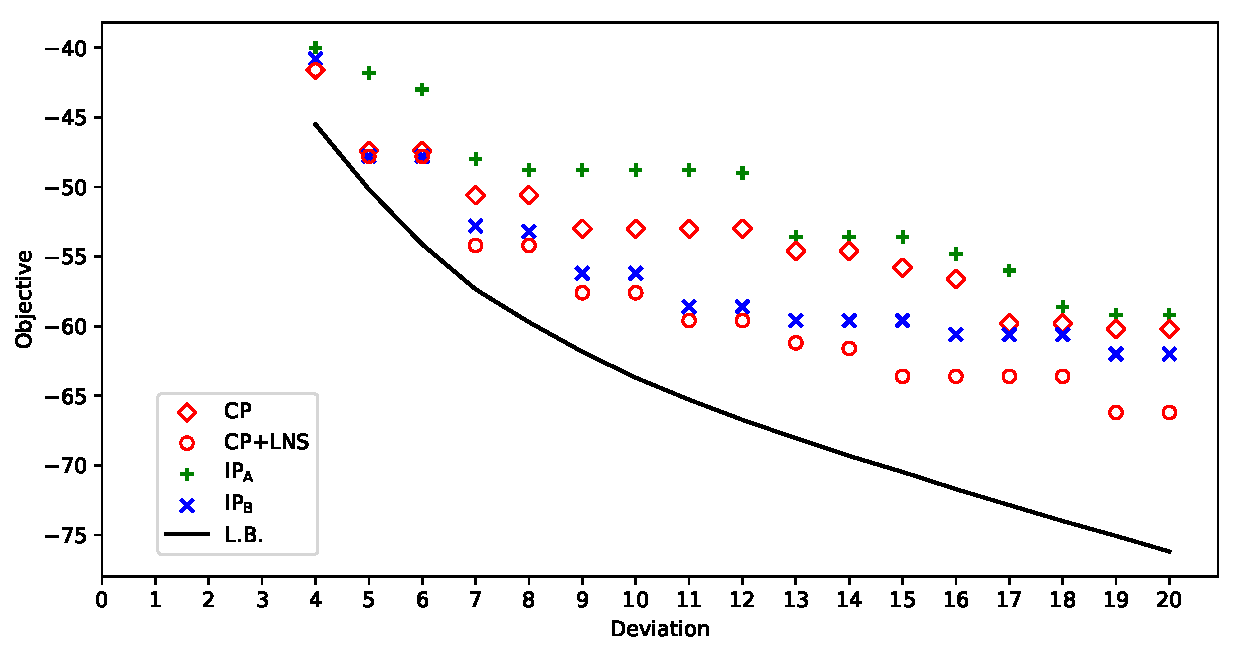
\includegraphics[scale=0.5]{results_25groups_tl600.pdf}
  \end{center}
  
\end{frame}


%---------------------------------------------------------------------------------------------------


\begin{frame}
  \frametitle{\AutoSectionTitle}
  \framesubtitle{50 groups, 6s time limit}

  \begin{center}
    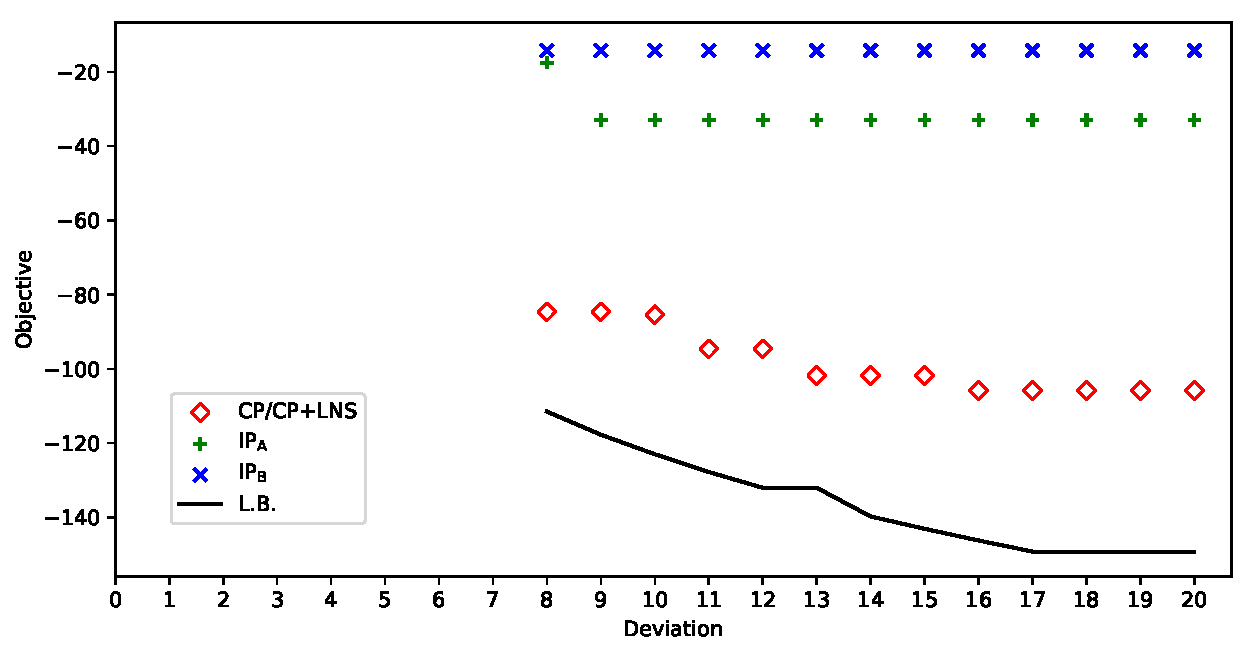
\includegraphics[scale=0.5]{results_50groups_tl6.pdf}
  \end{center}
  
\end{frame}


%---------------------------------------------------------------------------------------------------


\begin{frame}
  \frametitle{\AutoSectionTitle}
  \framesubtitle{50 groups, 600s time limit}

  \begin{center}
    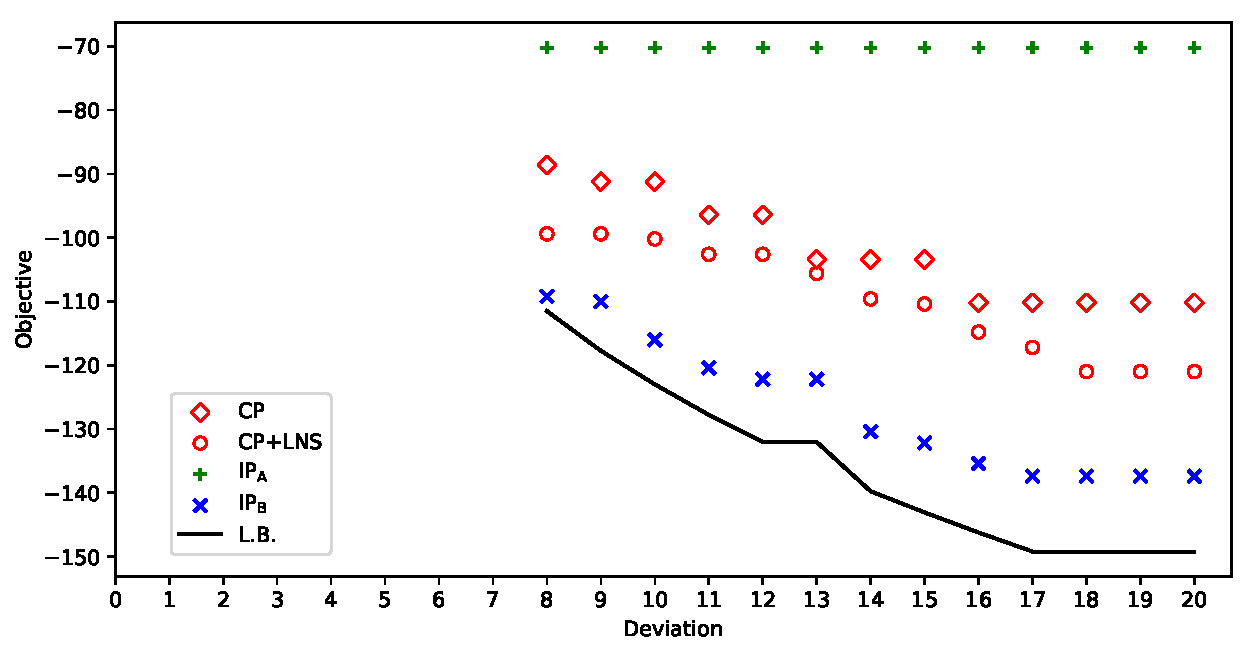
\includegraphics[scale=0.5]{results_50groups_tl600.pdf}
  \end{center}
  
\end{frame}


%---------------------------------------------------------------------------------------------------


\begin{frame}
  \frametitle{\AutoSectionTitle}
  \framesubtitle{50 groups, 600s time limit (costs only)}

  \begin{center}
    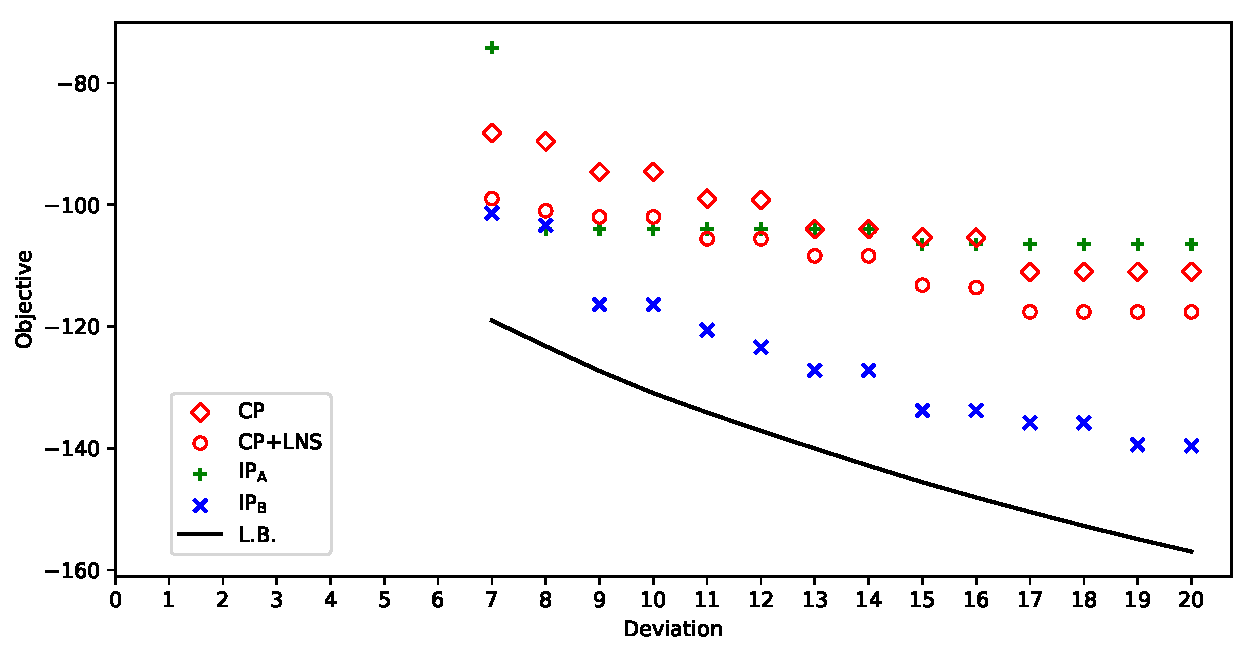
\includegraphics[scale=0.5]{results_costsonly_50groups_tl600.pdf}
  \end{center}
  
\end{frame}


%---------------------------------------------------------------------------------------------------


\begin{frame}
  \frametitle{\AutoSectionTitle}
  \framesubtitle{50 groups, 600s time limit (conflicts only)}

  \centering
  \begin{tabular}{lr}
    \cline{2-2}
    & \multicolumn{1}{c}{50 groups} \\
    \cline{2-2}
    & Conflicts only \\
    \hline
    CP                  & 0.03 \\
    CP+LNS              & 0.03 \\
    IP\textsubscript{A} & 601.11 \\
    IP\textsubscript{B} & 4.64 \\
    \hline
  \end{tabular}
  
\end{frame}


%---------------------------------------------------------------------------------------------------


\begin{frame}
  \frametitle{\AutoSectionTitle}
  \framesubtitle{Comparison With Metaheuristics}

  \begin{figure}[H]
    \begin{center}
      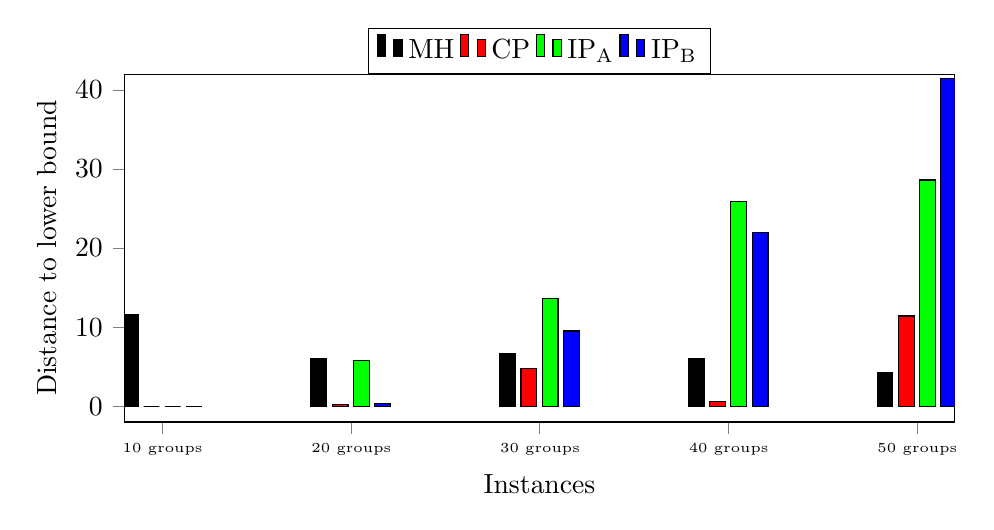
\begin{tikzpicture}
        \begin{axis}[
            ybar,
            width = \textwidth,
            height = 6cm,
            bar width = 2mm,
            enlargelimits=0.05,
            legend style={at={(0.5, 1)},
              anchor=south, legend columns=-1},
            ylabel={Distance to lower bound},
            xlabel={Instances},
            x tick label style={font=\tiny,text width=1cm,align=center},
            symbolic x coords={10~groups,20~groups,30~groups,40~groups,50~groups},
            xtick=data,
            ymin=0, ymax=40,
            ytick pos=left,
            ytick align=outside,
            xtick pos=bottom
          ]
          \addplot [fill=black] coordinates {(10~groups,11.6) (20~groups,6) (30~groups,6.6) (40~groups,6) (50~groups,4.2)};
          \addplot [fill=red] coordinates   {(10~groups,0) (20~groups,0.2) (30~groups,4.71) (40~groups,0.6) (50~groups,11.4)};
          \addplot [fill=green] coordinates {(10~groups,0) (20~groups,5.8) (30~groups,13.6) (40~groups,25.9) (50~groups,28.6)};
          \addplot [fill=blue] coordinates  {(10~groups,0) (20~groups,0.3) (30~groups,9.5) (40~groups,22) (50~groups,41.4)};
          \legend{MH, CP, IP\textsubscript{A}, IP\textsubscript{B}}
        \end{axis}
      \end{tikzpicture}
    \end{center}
  \end{figure}
  
\end{frame}


%% CONCLUSION %%%%%%%%%%%%%%%%%%%%%%%%%%%%%%%%%%%%%%%%%%%%%%%%%%%%%%%%%%%%%%%%%%%%%%%%%%%%%%%%%%%%%%


\renewcommand{\AutoSectionTitle}{Conclusion}

\section{\AutoSectionTitle}

\begin{frame}
  \frametitle{Outline}
  \tableofcontents[currentsection]
\end{frame}


%---------------------------------------------------------------------------------------------------


\begin{frame}
  \frametitle{\AutoSectionTitle}
  \framesubtitle{Metaheuristics Model}

  \begin{itemize}
  \item[$+$] Good early solutions \\~\\
  \item[$+$] Scales well \\~\\~\\~\\~\\

    \pause
    
  \item[$-$] No proof of optimality \\~\\    
  \item[$-$] Poor balance
  \end{itemize}

\end{frame}


%---------------------------------------------------------------------------------------------------


\begin{frame}
  \frametitle{\AutoSectionTitle}
  \framesubtitle{CP Model}

  \begin{itemize}
  \item[$+$] Very good early solutions \\~\\
  \item[$+$] Proves optimality for small instances \\~\\
  \item[$+$] Quickly proves optimality or infeasibility for all instances when there are no costs \\~\\~\\~\\~\\

    \pause
    
  \item[$-$] Hard to optimize with costs \\~\\
  \item[$-$] Limited symmetry breaking
  \end{itemize}

\end{frame}


%---------------------------------------------------------------------------------------------------


\begin{frame}
  \frametitle{\AutoSectionTitle}
  \framesubtitle{IP Model A}

  \begin{itemize}
  \item[$+$] Simple model \\~\\
  \item[$+$] Proves optimality for small instances \\~\\~\\~\\~\\

    \pause
    
  \item[$-$] Inefficient \\~\\
  \item[$-$] Limited symmetry breaking
  \end{itemize}

\end{frame}


%---------------------------------------------------------------------------------------------------


\begin{frame}
  \frametitle{\AutoSectionTitle}
  \framesubtitle{IP Model B}

  \begin{itemize}
  \item[$+$] Near-optimal solutions \\~\\
  \item[$+$] No symmetry \\~\\
  \item[$+$] Provides a good lower bound \\~\\~\\~\\~\\

    \pause
    
  \item[$-$] Complex \\~\\
  \item[$-$] No proof of optimality \\~\\    
  \item[$-$] Poor early solutions
  \end{itemize}

\end{frame}


%---------------------------------------------------------------------------------------------------


\begin{frame}
\end{frame}


%%%%%%%%%%%%%%%%%%%%%%%%%%%%%%%%%%%%%%%%%%%%%%%%%%%%%%%%%%%%%%%%%%%%%%%%%%%%%%%%%%%%%%%%%%%%%%%%%%%%


\end{document}
